\documentclass[11pt,a4paper]{scrartcl}
\usepackage[ngerman]{babel}
\usepackage[utf8]{inputenc}
\usepackage[T1]{fontenc}
\usepackage{graphicx}
\usepackage{float}
\usepackage{fullpage}
\usepackage{amssymb}
\usepackage{amsmath}
\usepackage[nounderscore]{syntax}
\usepackage{url}                % URLs
\usepackage{tikz}               % for the grey border on the title page
\usepackage{ziffer}				% to use commas as decimal separators in math mode
\usepackage{pdflscape}
\usepackage{multirow}
\usepackage{booktabs}
\usepackage{longtable, mdwtab}
\usepackage[absolute,overlay]{textpos}

\usepackage[a4paper,left=40mm,right=30mm,top=20mm,bottom=20mm,includeheadfoot]{geometry}
\newcommand{\changefont}[3]{\fontfamily{#1} \fontseries{#2} \fontshape{#3} \selectfont}
\parindent 0pt
\usepackage[raiselinks=true,
						bookmarks=true,
						bookmarksopenlevel=1,
						bookmarksopen=true,
						bookmarksnumbered=true,
						hyperindex=true,
						plainpages=false,
						pdfpagelabels=true,
						pdfborder={0 0 0.5},
						colorlinks=false,
						linkbordercolor={0 0.61 0.50},
						citebordercolor={0 0.61 0.50}]{hyperref}  %{0.57 0.74 0.57}

\author{PSE-Projekt 4 Team 2}
\title{Entwurfsdokument zu Worthwhile}

\setcounter{tocdepth}{1} % make TOC fit on one page

\hyphenation{Worth-while}

\newcommand{\reqtype}{}
\newenvironment{reqlist}[1]{\begin{description} \renewcommand{\reqtype}{#1}}{\end{description}}
\newcommand{\req}[3]{\item[\textbf{/\reqtype{}#1/}] #2 \\ #3}
\newcommand{\see}[1]{#1}
\renewcommand{\int}{\texttt{Integer}}
\newcommand{\bool}{\texttt{Boolean}}

\newcommand{\method}[1]{
			\item[\texttt{\textbf{#1}}]
            }
\newcommand{\attr}[1]{\item[\texttt{\textbf{#1}}]}
\newcommand{\type}[1]{\texttt{#1}}
\newcommand{\literal}[1]{\item[\texttt{#1}]}
\newcommand{\mlmethod}[1]{\method{\parbox{\textwidth}{#1}}}
\newenvironment{rcases}{%
  \left.\renewcommand*\lbrace.%
  \begin{cases}}%
{\end{cases}\right\rbrace}
\graphicspath{{images/}}

\begin{document}

%% titlepage.tex
%%

% coordinates for the bg shape on the titlepage
\newcommand{\diameter}{20}
\newcommand{\xone}{-30}
\newcommand{\xtwo}{150}
\newcommand{\yone}{15}
\newcommand{\ytwo}{-265}

\begin{titlepage}
% bg shape
\begin{tikzpicture}[overlay]
\draw[color=gray]
 		 (\xone mm, \yone mm)
  -- (\xtwo mm, \yone mm)
 arc (90:0:\diameter pt)
  -- (\xtwo mm + \diameter pt , \ytwo mm)
	-- (\xone mm + \diameter pt , \ytwo mm)
 arc (270:180:\diameter pt)
	-- (\xone mm, \yone mm);
\end{tikzpicture}

	\begin{textblock}{10}[0,0](1.7,1)
		
\includegraphics[width=.3\textwidth]{images/kit_logo_de_4c_positiv.pdf}
	\end{textblock}
	\changefont{phv}{m}{n}	% helvetica	
	\begin{center}
		\fontsize{45}{50}\selectfont
        \vfill
        \textsc{Worthwhile} \\
        \textsc{Pflichtenheft}
        \vfill
		\LARGE
		PSE WS 11/12
  \vfill
 \newpage
 
 \null
 \vfill
 
 Praxis der Softwareentwicklung -- WS 2011/2010 \\
  Automatisches Prüfen der Korrektheit von Programmen \\
  Projekt 4 -- Gruppe 2 \\
  \medskip
  \vspace{2cm}
  \Large
  \begin{tabular}{|l|l|}
    \hline
    Leon Handreke & 123456 \\
    \hline
    Chris Hiatt & 1610922 \\
    \hline
    Stefan Orf & 123456 \\
    \hline
    Joachim Priesner & 1579308 \\
    \hline
    Fabian Ruch & 123456 \\
    \hline
    Matthias Wagner & 1579342 \\
    \hline
  \end{tabular}
  \vspace{2cm} \\
  \today \\
	Revision 0
	\end{center}
	
  \vfill

\end{titlepage}


\tableofcontents
\clearpage

\section{Zeitlicher Ablauf}

Im Großen und Ganzen hat sich die Zeitplanung aus der Entwurfsphase bewährt. Die Aufteilung in Aufgabenbereiche wurde weitestgehend eingehalten. Während der Entwicklung hat es sich als vorteilhaft erwiesen, eng ineinandergreifende Komponenten parallel zu entwickeln, um den geschriebenen Code sofort testen zu können. Im aktualisierten Gantt-Diagramm erscheinen deshalb einige Einheiten deutlich größer. Tatsächlich hat sich aus der Parallelisierung kein höherer Zeitaufwand ergeben. Trotzdem haben sich einige kleinere Änderungen im Laufe der Implementierungsphase ergeben, welche im Folgenden genauer dargestellt werden.

\subsection{Build-System}
Die Inbetriebnahme des Build-Systems sowie des Continous-Integration-Servers hat sich aufgrund einiger Schwierigkeiten bei der Konfiguration um einige Tage in die Weihnachtsferien hinein verschoben.

\subsection{Stubs und Unit-Tests}
Ursprünglich war geplant, vor der eigentlichen Implementierung Unit-Tests zu erstellen und die Klassen mit Stubs auszurüsten, welche die Tests erfolgreich ablaufen lassen. Da das Parsen von Testprogrammen jedoch bereits früh möglich war, wurden stattdessen parallel zur Implementierung Unit-Tests mit an den Testfall angepassten Testprogrammen geschrieben.

\subsection{Parser}
Aufgrund der Entscheidung, keine eigene Schnittstellenklasse zum Parser zu implementieren (siehe \ref{aenderung_parser}), sondern die von ANTLR generierte Klasse direkt zu verwenden, entfiel diese Aufgabe.

\subsection{Beweiserschnittstelle}
Die Abhängigkeit zwischen den Aufgaben "`Z3-Anbindung"' und "`SMTLIB-Kompilierung"' wurde aufgelöst, da es sich als vorteilhaft für die Zeiteinteilung herausstellte, beide parallel zu der aufwendigeren Formelgenerierung zu entwickeln.

\subsection{Interpreter}
Der Entschluss, alle Debug-Logik in einer seperaten "`Debugger"'-Komponente zu implementieren (siehe \ref{aenderung_interpreter_breakpoints}), führte dazu, dass die Einheit "`Breakpoints"' vom Aufgabenbereich "`Interpreter"' in den Aufgabenbereich der GUI-Entwicklung verschoben wurde.

\begin{landscape}%
	\begin{figure}%
		\vspace{-2cm}
		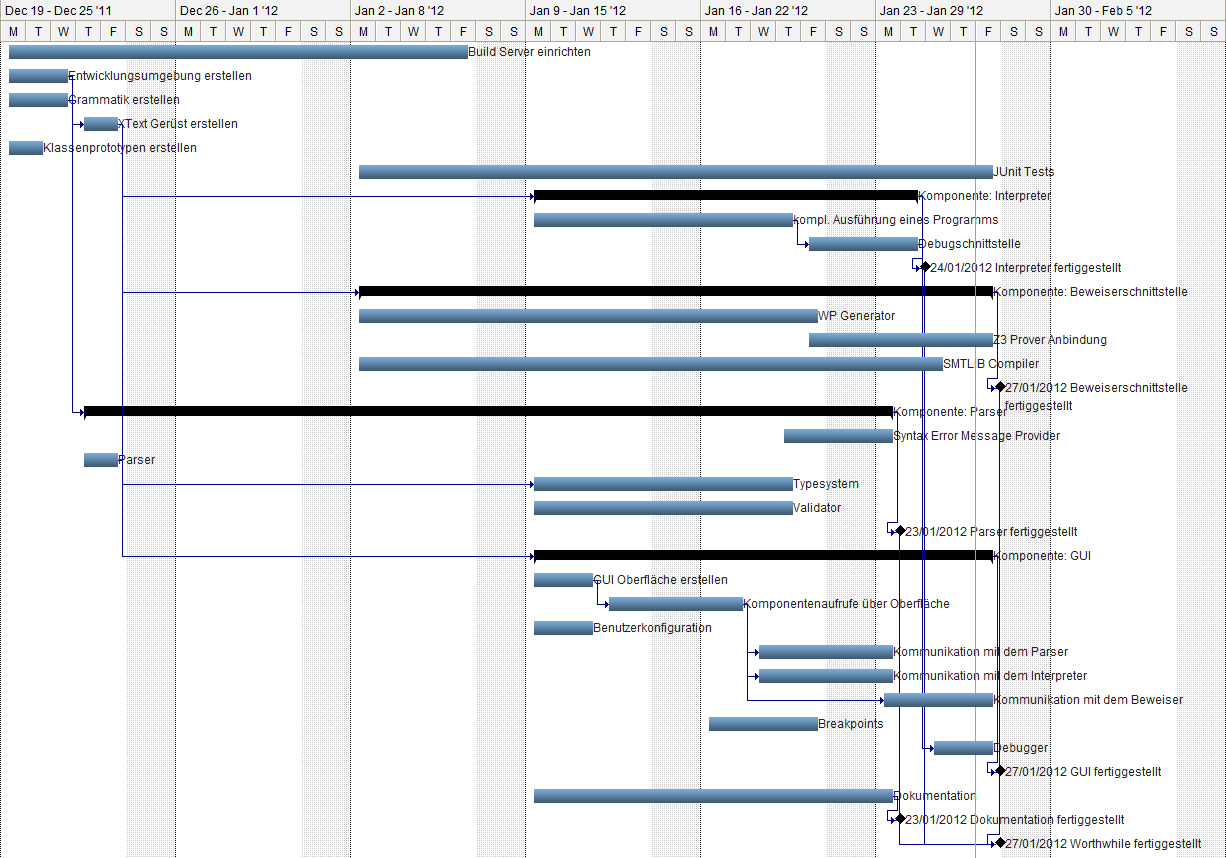
\includegraphics[height=1.2\textheight]{images/gantt_implementierung_diag.png}%
		\caption{Tatsächlicher Ablauf der Implementierungsphase.}%
	\end{figure}%
\end{landscape}

\section{Änderungen am Entwurf}
% TODO: generelle Einführung, wie toll unser Entwurf doch war
\subsection{Grammatik}
In der Grammtik wurde das neue Schlüsselwort \texttt{\_return} eingefügt, um auf den Rückgabewert einer Funktion in ihrer Nachbedingung zugreifen zu können.

\subsection{Parser}
\subsection{Interpreter}
\subsection{Beweiserschnittstelle}
\subsection{GUI}


\clearpage
\appendix

\end{document}
